%Problemet med sidekanaler (skal lede op til baggrundsafsnittet)
%Nævn evt. også noget om små devices.

% Motivation
For the last hundred years or so, the only way to intercept encrypted messages between parties has been to break the encryption algorithm with crypto analysis. As a result, some very robust cryptography algorithms has been developed that are very hard to attack.
Instead of attacking the algorithm, recent research has focused on vulnerabilities related to the devices that communicate.
It is possible to learn a lot about the data or the algorithm simply from measuring the device on which it resides. Heat generation, time, sound etc. are all components of the cryptograpic event that happened and tell part of the story.
These vulnerabilities are called ``side-channel``-vulnerabilities because they are not directly related to the cryptography algorithms, but rather a byproduct.

And while strong cryptographic methods such as AES (encryption), SHA-256 (hashing) and RSA/Elliptic Curve (signing) work well on systems with reasonable processing power and memory capabilities, they do not scale well into a world with embedded systems and sensor networks.
This introduces some challenges such as how to reduce the amount of costly operations whilst still guaranteeing the highest level of security.
The limits related to physical size, processing power, memory and battery life call for more lightweight cryptography methods to be implemented on such systems.
Lightweight cryptography applications can be implemented in many programming languages, most of which still leave the devices open to side-channels.
The good news is that some of these side-channels are, at least in theory, avoidable if we choose our language of implementation carefully.
One such class of languages are reversible languages, which we will expand on in the following section before coming back to side-channels in Chapter ~\ref{chapt - Side-channel}.

%While conventional cryptography methods, such as AES (encryption), SHA-256 (hashing) and RSA/Elliptic Curve (signing) work well on systems with reasonable processing power and memory capabilities, these do not scale well into a world with embedded systems and sensor networks.
%This introduces some challenges such as how to reduce the amount of costly operations whilst still guaranteeing the highest level of security. The limits related to physical size, processing power, memory and battery life call for more lightweight cryptography methods to be implemented on such systems.
%Lightweight cryptography applications can be implemented in many programming languages, most of which still leave the devices open to more sophisticated hacking methods such as timing attacks.
%These sophisticated hacks exploit weaknesses in physical "side-channels" and are, at least in theory, avoidable if we choose our language of implementation carefully.
%We will expand on reversible computing first, and then come back to side-channels in Chapter ~\ref{chapt - Side-channel}.

\section{Reversible Programming}
% NAND gates are irreversible.
% Landaurs principle is that heat must be generated when doing any "logically irreversible manipulation of information".
Reversible programs can be run both forwards and backwards deterministically, calculating output from input as well as input from output.
What this means is that all functions are bidirectional, i.e. given some resulting output of a function, we can run the inverse of that function with the output and find the initial input.
This is especially useful with algorithms for encryption or encoding, where an inverse process is most often needed.
If implemented without too much overhead, this will result in smaller programs, as the encoding/encryption function is bidirectional and can be used for decoding/decryption as well.

Writing code in a language where all functions are bidirectional imposes some constraints on the programmer: variables local to a function must be initialized as zero and reset to zero after use.
All variable updates must be lossless, therefore not allowing modulo updates such as \lstinline{x = x mod y} as there is no inverse to this operation.
Bit-shift operations must also be lossless, i.e. when bits are rotated off the right end, they are inserted into the vacated bit positions on the left and vice-versa. While imposing some restrictions on the programmer, reversible programming languages has a lot to offer in terms of security: they ensure no loss of information and no variables are left in memory after a program has run, since all variables are reset after use. Thus the memory will not contain any data that can be used for side-channel attacks such as information leakage.

\section{Foundations for this work}
This Master thesis revolves around the reversible programming language Hermes developed at DIKU.
Hermes is based on the reversible programming language Janus and designed specifically for writing encryption algorithms\cite{MogensenHermes}.
By virtue of some carefully thought-out design choices, Hermes offers a built-in protection against some side-channel attacks such as information leakage.

Figure~\ref{fig:compilationProcess} is a visualization of the entire project. It shows the current implementation marked with red and the contributions of this thesis marked with green. This thesis focuses on ARM64 as target language, but other target languages could be added as future work. Two examples of such target languages are added and marked with a dotted line.
\begin{figure}[tp]
  \centering
  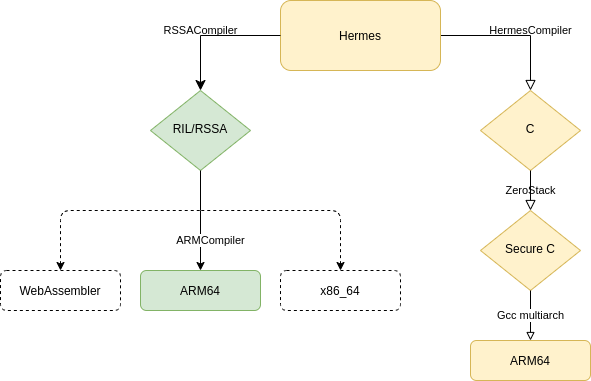
\includegraphics[scale=0.57]{Graphics/compilationProcess.png}
  \caption{Visualization of the project}
  \label{fig:compilationProcess}
\end{figure}

There are a few problems with Hermes in its current implementation, where Hermes programs are translated to C by the program \emph{hc} and then to assembly code with the GNU Compiler Collection (gcc).
We do not have full control over everything that happens in the gcc compiler and gcc does not prevent side-channel attacks, such as information leakage and timing attacks\cite{Simon2018}.
One can use zerostack\cite{Github.zerostack} to zero out the stack and registers of sensitive functions, but this process is very cumbersome and has not yet been thoroughly tested. 
Protection against side-channel attacks would be much easier to enforce with a compilation directly to assembly language, which is the primary focus of this Master thesis.
When we are able to compile directly from Hermes to assembly it will allow us to modify the translation to ensure protection and make it much easier to extend the implementation to other target assembly languages such as WebAssembly or x86\_64.
We make use of the Reversible Single Static Assignment (RSSA) representation from \cite{10.1007/978-3-319-41579-6_16}, which describes how to combine Single Static Assignment (SSA) with Reversible Intermediate Language (RIL) to obtain RSSA.
Furthermore we implement the lightweight cryptography algorithm Twofish in Hermes based on the implementation from the original authors of the algorithm \cite{GIT2F}. We use benchmarks to argue for the correctness of both implementations.



